\cbox{Section word count: 1400}

\subsection{WasteAndMaterialFootprint tool}\label{sec:results-wmf}
We have written an extension to the brightway2 LCA framework that calculates the waste footprint of a product or service.
It finds upstream waste flows in a supply chain, categorises waste flows into 14 types and finds hotspots in waste generation.
It explodes the database, identifies upstream waste exchanges, edits them and writes custom WasteFootprint methods. The waste flows then become pseudo-biosphere flows and the waste footprint can be calculated as an LCIA method. The WasteFootprint tool can be easily applied to calculate the `footprints' of other supply-chain flows such as water, gas, and critical raw materials.

In the context of environmental impact assessments, where a variety of indicators have been proposed and debated for their significance and communicability \citep{vanham2019footprints,ridoutt2013footprints}, the WasteAndMaterialFootprint (WMF) tool serves to re-simplify environmental decision-making. This tool leverages the findings that a limited set of indicators can cover a significant portion of environmental impact variance \citep{steinmann2017resourcefootprints}, enabling more streamlined and effective assessment processes.

\subsubsection{Waste exchanges}\label{sec:results-wmf-waste_exchanges}

In LCA waste flows are not considered as fundamental biosphere exchanges, but rather as technosphere flows. Waste produced by an activity is transferred to a relevant waste treatment activity where it is accepted `burden-free' and transformed into a combination of emissions and other waste `products'~\citep{guinee2021wasteisnotaservice}. There can be several treatment steps in this pathway leading, ultimately, to a mass of material being deposited in a landfill. In this system of waste accounting, the impacts apportioned to the waste-producing activity are a sum of those incurred by the transport, treatment, and final disposal of the waste into terrestrial or aquatic environments. In particular, the extensive work of~\cite{doka2024publications} has contributed significantly to understanding the environmental impacts of waste treatment processes and the long-term impacts of disposal. 

The purpose of the WMF tool is not to quantify the environmental impacts of waste treatment, but rather to quantify the waste flows themselves, even those that are finally consumed by waste treatment processes. It provides, thus, not an impact assessment in the traditional sense, but an accounting of the waste generated by a product or service, regardless of the end-of-life fate of these flows. By definition, the development of the `circular economy' necessitates the reduction and ultimate elimination of waste---though whether this objective is thermodynamically impossible has long been the subject of lively debate by~\cite{ayres1998recycling},~\cite{reuter2012recyclinglimits} and many others. In any case, waste avoidance is of critical importance and by quantifying and classifying the waste total attributed to a product or service in an LCA database, the WMF tool provides a practical means to identify hotspots and opportunities for waste reduction and efficiency.

The logic of screening for waste exchanges is based on a set of boolean search queries (`AND', `OR', and `NOT') that are applied in a list comprehension to the names of every exchange in the LCA database (see `search\_queries.py' for the full list). In this way, the search queries enable classification into categories (such as `hazardous solid' and `incineration liquid') and permit the identification of waste exchanges in addition to those directly connected to waste treatment processes. The search queries are tailored to the specific database and the user can easily modify them to suit their needs. In the default settings, there are a total of 18 waste classifications (9 categories, each separated into liquid and solid waste) For example, the identification of `non-hazardous solid' waste exchanges is based on the following search query; \texttt{AND = [`waste'], NOT = [`hazardous', `radioactive'], UNIT = [`kilogram']} (this can also be inferred and confirmed by comparison with the difference between the results of `total solid' and `hazardous solid').\ \autoref{tab:wf_results} presents a list of waste exchanges identified in the prospective database built from `ecoinvent 3.9.1' according to the IAM model `REMIND' with the RCP `PkBudg500' in the year 2100. Note that for prospective databases, a waste category for `carbon dioxide' has been created to account for the carbon capture and storage (CCS) that has been implemented in this model. 

\begin{table}[ht]
    \centering
    \caption{WasteFootprint search results for the database `ecoinvent cutoff 3.9.1, REMIND, SSP2, PkBudg500, 2100'.}\label{tab:wf_results}
    \begin{tabular}{llr}
        \toprule
        \textbf{Waste exchanges} & \textbf{Unit} & \textbf{Exchange count} \\
        \midrule
        digestion & kilogram & 4 \\
        composting & kilogram & 26 \\
        open burning & kilogram & 535 \\
        incineration & kilogram & 2171 \\
        recycling & kilogram & 137 \\
        landfill & kilogram & 1530 \\
        hazardous & kilogram & 1928 \\
        carbon dioxide & kilogram & 119 \\
        total & kilogram & 29524 \\
        digestion & cubic meter & 16 \\
        composting & cubic meter & 0 \\
        open burning & cubic meter & 0 \\
        incineration & cubic meter & 2 \\
        recycling & cubic meter & 0 \\
        landfill & cubic meter & 2 \\
        hazardous & cubic meter & 437 \\
        carbon dioxide & cubic meter & 0 \\
        total & cubic meter & 4360 \\
        \bottomrule
\end{tabular}
\end{table}

\subsubsection{Material exchanges}\label{sec:results-wmf-material_exchanges}

The logic for the identification of material exchanges with the WMF tool differs from that used to identify waste exchanges in that the search queries are based on the names of the so-called relevant `market activities' for the material of interest. That is, for material $x$, all exchanges with the name `market for material $x$' are identified and subsequently apportioned a (`pseudo-biosphere') material demand exchange of the same sign and magnitude as the original exchange. A useful feature of the WMF tool is that, in cases where there are several markets for one material or material group, the program can easily aggregate these exchanges. For example, exchanges with markets for the rare-earth-elements (REEs) `market for cerium', `market for dysprosium', `market for erbium', etc.\ can be aggregated into a single indicator category for REEs. Similarly, the total demand for all critical raw materials (CRMs) can be easily calculated in the same manner. 

As discussed in the introduction~\ref{sec:introduction} there are some existing material demand methods in the standard LCIA method sets, including the `crustal scarcity indicator' (which provides only an aggregated, abstracted endpoint)~\citep{arvidsson2020csi} and the (deprecated) EDIP 2003 material use indicators (which provide endpoints in fundamental units)~\citep{hauschild2003edip}. In these methods, the material demand is calculated based on the total mass that is extracted from the environment, thus, their focus is essentially solely on the mining-related exchanges that bring these materials from the biosphere into the technosphere. In the WMF tool, however, the accounting for material demand is based on exchanges solely within the technosphere. This offers a different perspective, allowing for the estimation of overall supply-chain material demands that consider the entire life cycle of an activity, including non-direct impacts on the market such as co-production of other materials. Consider a demand for an activity containing a metal, for example; while the existing material use methods allow one to calculate the total mass of that metal that is extracted from the environment, the WMF tool can provide insight into the broader supply-chain impacts of the demand for this metal. If the production other materials are attributed to the production of this metal, these would appear as negative material demands in the WMF results---supply chain pressure for one material can result in lessening of supply chain pressure for another. In the results of the Li-ion battery case study in \autoref{sec:results-case_study}, we will see that this is indeed the case for the demand for nickel, which, because of such effects, is counter-intuitively negative despite the presence of nickel in the final products.


\subsection{Case study: Li-ion batteries}\label{sec:results-case_study}


As listed in \autoref{sec:method-case_study}, this case study calculated the waste and material footprints (as well as a variety of other indicators) for the unaltered inventories for five Li-ion batteries with the functional unit being 1~kg of battery. The purpose of this simple case study was to test, verify, and demonstrate the functionality and limitations of the WMF tool. This section includes some highlights of the results and the full results are available in the supplementary material.

\subsubsection{Temporal and scenario variation in waste and material footprints}\label{sec:results-case_study-total_footprints}

\autoref{fig:waste_total} shows the total solid waste footprint for the five Li-ion batteries in the case study from 2020 to 2100 under the SSP2 scenario using the baseline and PkBudg500 RCPs of the REMIND model. The NMC811 battery has the largest footprint, producing over 50~kg of waste per kilogram of battery produced. The LiMn2O4 battery has the smallest footprint, producing less than 4~kg of waste per kilogram of battery. In each case there was a slight downward trend in the waste footprints between 2020 and 2100. This is most notable in the period between 2020 and 2040 and is attributable to the relatively rapid decrease in fossil-fuel use that is included in the models over this time. For the total waste generated by these batteries, there was very little difference observed between the baseline and PkBudg500 RCPs.


\begin{figure}[ht!]
    \centering
    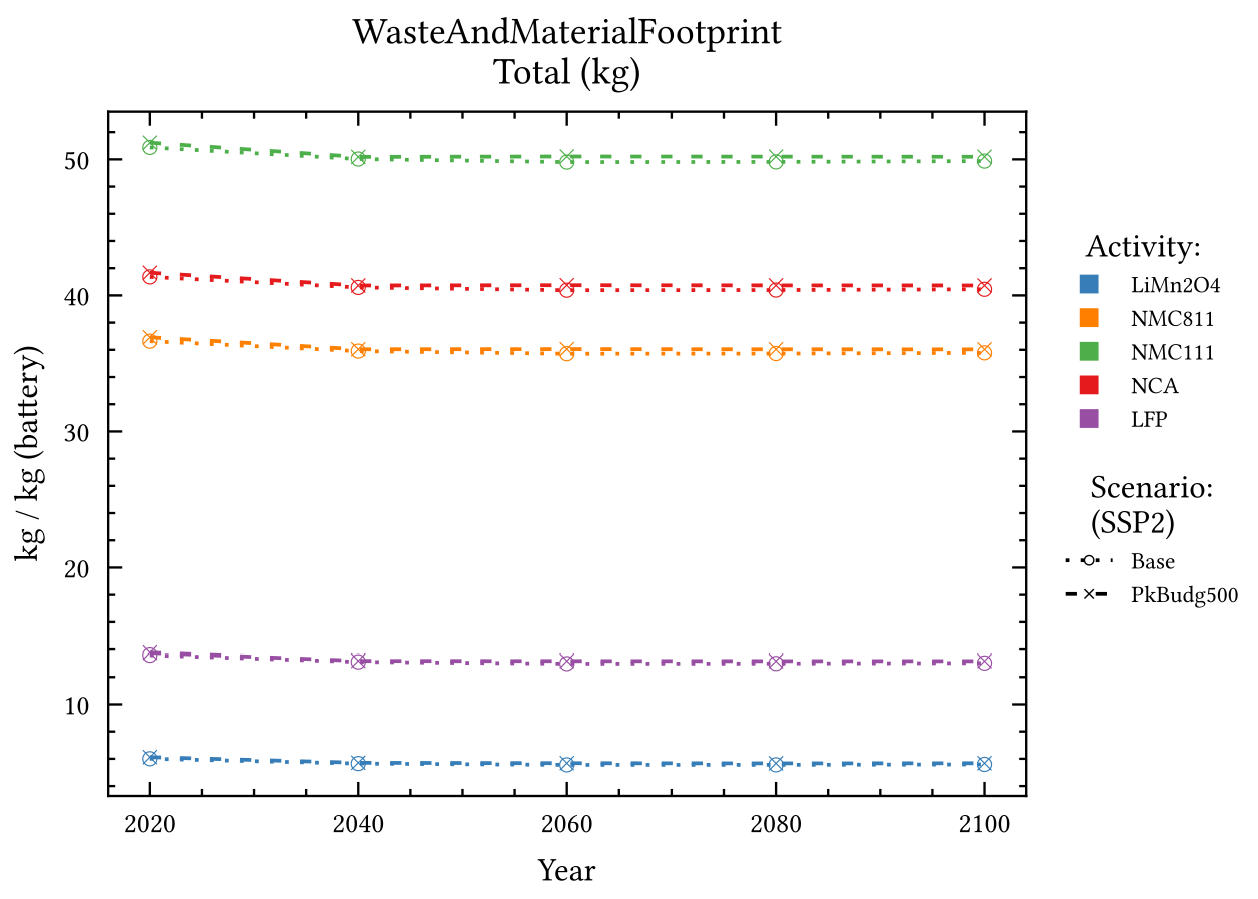
\includegraphics[width=\linewidth]{figures/total_waste.png}
    \caption{Total solid waste footprints for the five Li-ion batteries in the case study from 2020 to 2100 under the SSP2 scenario using the baseline and PkBudg500 RCPs of the REMIND model.}\label{fig:waste_total}
\end{figure}

The inclusion of carbon capture and storage in the prospective databases using the PkBudg500 RCP is evident in \autoref{fig:carbondioxide}, which shows a rapid increase in the production of carbon dioxide `waste' over the period from 2020--2040 that is not seen in the baseline.


\begin{figure}[ht!]
    \centering
    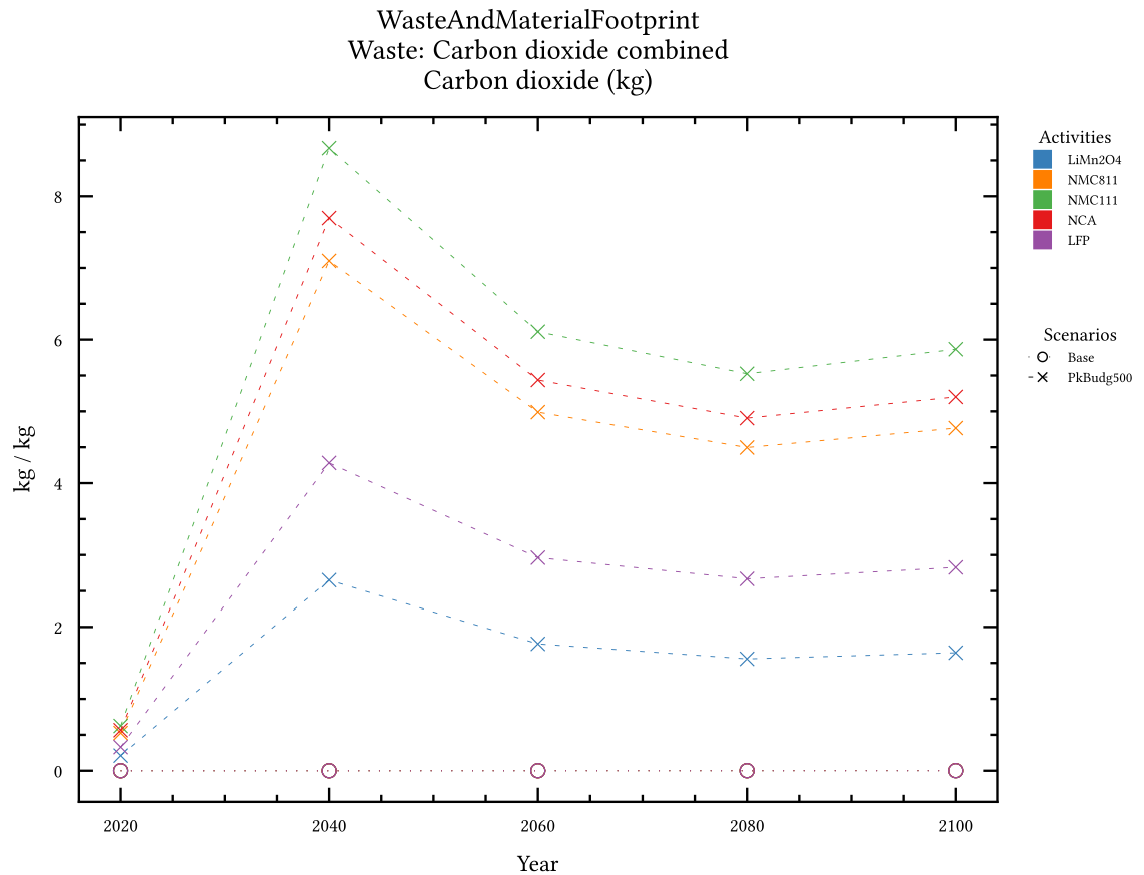
\includegraphics[width=\linewidth]{figures/carbondioxide.png}
    \caption{Carbon dioxide waste (from carbon capture and storage) footprints for the five Li-ion batteries in the case study from 2020 to 2100 under the SSP2 scenario using the baseline and PkBudg500 RCPs of the REMIND model.}\label{fig:carbondioxide}
\end{figure}

For the phosphate demand footprints that are depicted in \autoref{fig:phosphate}, the LFP (lithium iron phosphate) battery has a much larger footprint than the other batteries, consistent with its composition. In this case, the phosphate footprint of all batteries is shown to decrease over the period from 2020--2100, and the RCP scenarios are seen to converge between 2020 and 2040.

\begin{figure}[ht!]
    \centering
    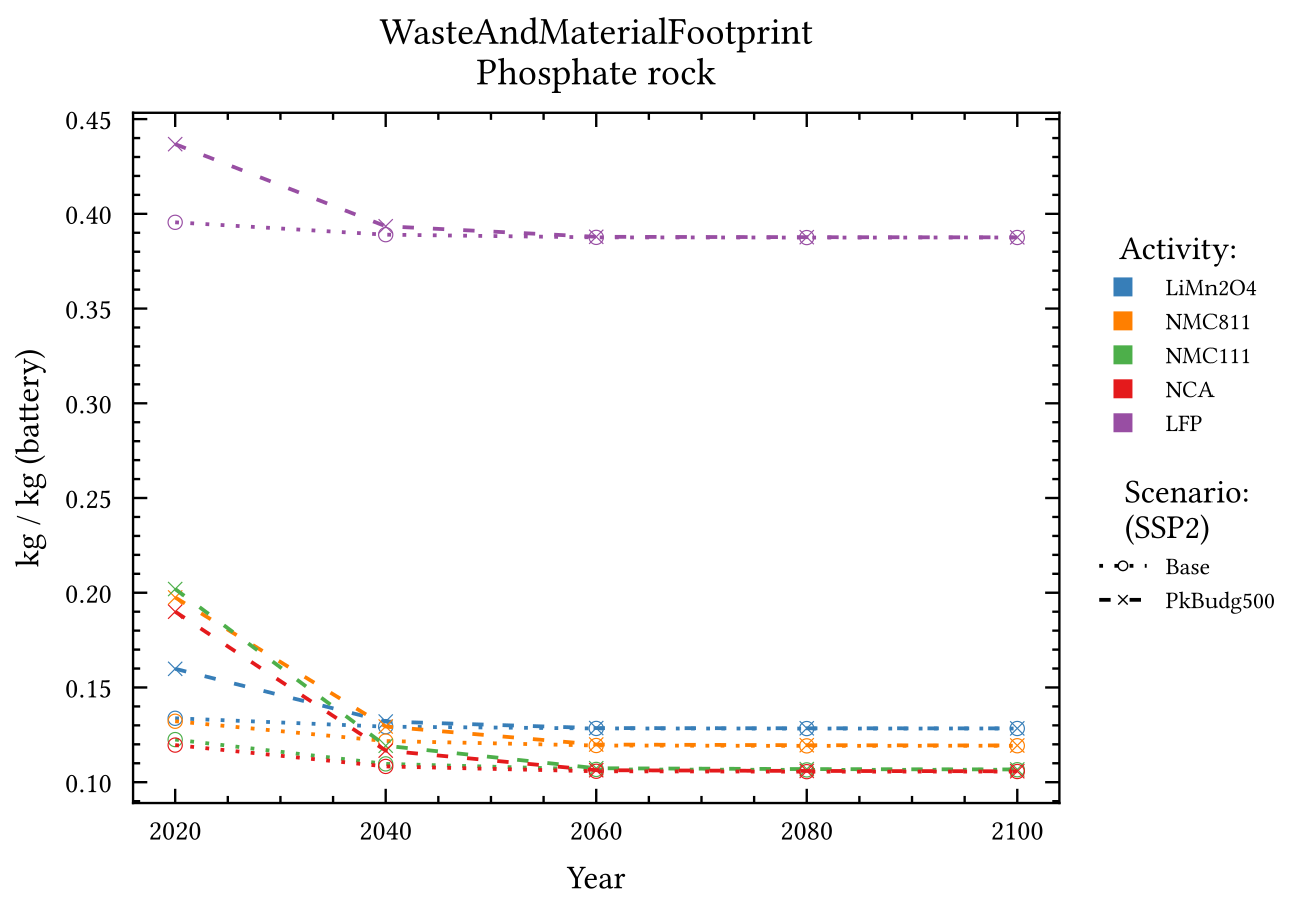
\includegraphics[width=\linewidth]{figures/phosphate.png}
    \caption{Phosphate material demand footprints for the five Li-ion batteries in the case study from 2020 to 2100 under the SSP2 scenario using the baseline and PkBudg500 RCPs of the REMIND model.}\label{fig:phosphate}
\end{figure}

\subsubsection{Contribution of `top-processes' in the supply chain}\label{sec:results-case_study-topprocesses}

\autoref{fig:top_contribution} shows the contribution of the `top-processes' to the cobalt footprint of the LiMn2O4 battery under the baseline scenario from 2020--2100. The total footprint is seen to almost triple, from 2.2~kg/kg in 2020 to 6.2~kg/kg in 2100. This result is likely a reflection of the electrification of the transport sector that is included in the REMIND model. The fractional contributions of the top processes is remains relatively steady over the coming century in this case. 

\begin{figure}[ht!]
    \centering
    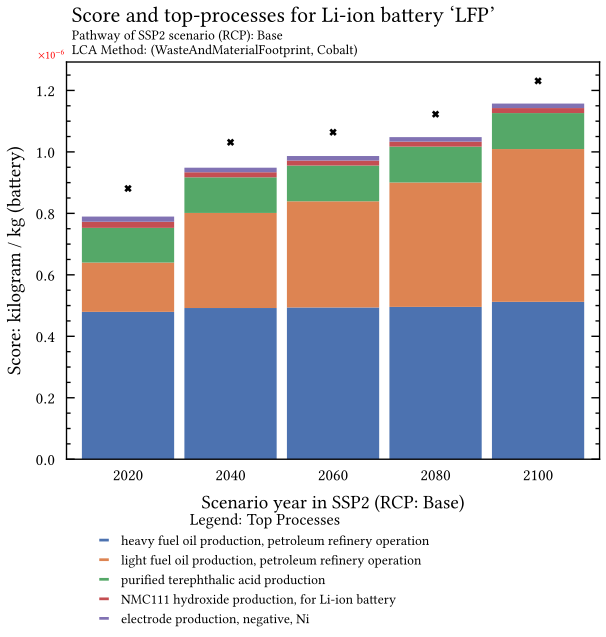
\includegraphics[width=0.8\linewidth]{figures/top-processes.png}
    \caption{Contribution of `top-processes' to the case study from 2020 to 2100 under the SSP2 scenario using the baseline and PkBudg500 RCPs of the REMIND model.}\label{fig:top_contribution}
\end{figure}

\subsubsection{Contribution of industrial sectors in the supply chain}\label{sec:results-case_study-topsectors}

\autoref{fig:cpc_contribution} shows the contribution of industrial sectors (grouped by CPC classifications) to the total liquid waste footprint of the NCA battery under the PkBudg500 pathway.

\begin{figure}
    \centering
    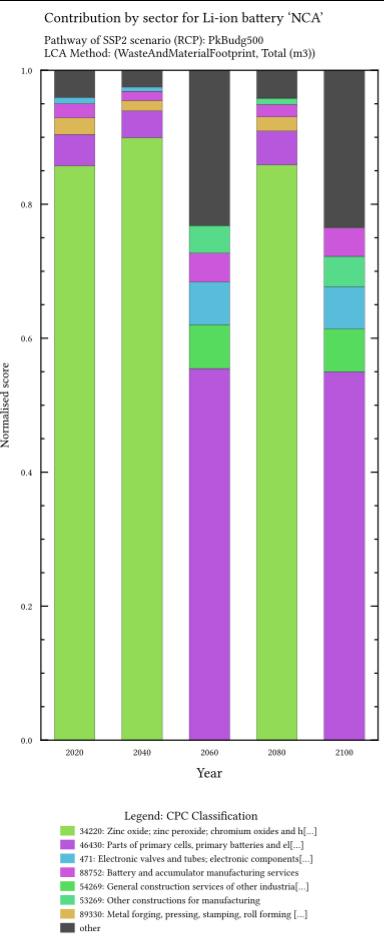
\includegraphics[width=0.8\linewidth]{figures/cpc_contribution.png
    }
    \caption{Contribution of industrial sectors to the liquid waste footprint of the NCA battery from 2020 to 2100 under the SSP2 scenario using the PkBudg500 RCP of the REMIND model.}\label{fig:cpc_contribution}
\end{figure}